\documentclass[10pt]{article}   % document properties
\usepackage[spanish]{babel}     % spanish package
\usepackage[utf8]{inputenc}     % codificacion de caracteres utf-8
\usepackage[top=2.3cm,bottom=3.5cm,right=2.5cm,left=2.5cm]{geometry}   % modify margins 
\usepackage{multicol}           % multiple columsn
\usepackage{graphicx}           % manage images 
\usepackage{url}                % manage aesthetic links
\usepackage{hyperref}           % internal links and more
\usepackage{array}              % customize tables         
%\usepackage{tcolorbox}          % colorful boxes
\usepackage{caption}            % improve figures & tables captions
\usepackage{tabularx}           % table advanced (sized)
\usepackage{lipsum}             % lipsum text
\usepackage{fancyhdr}           % headers and footers
\usepackage{xcolor, colortbl}   % define customize colors & table colore
\usepackage{listings}           % show & customize code
%%%%%%%%%%%%%%%%%%%%%%%%%%%%%%  extra definitions  %%%%%%%%%%%%%%%%%%%%%%%%%%%%%%%
\lstdefinestyle{ascii-tree}{
	literate={├}{|}1 {─}{--}1 {└}{+}1 
}
\newcolumntype{M}[1]{>{\centering\arraybackslash}m{#1}}     % cell configuration
\pagestyle{fancy}               % choosing fancy style
\fancyhf{}                      % delete any footer or header
\renewcommand{\headrulewidth}{0pt} % delete header line
% para el codigo fuente
\definecolor{dkgreen}{rgb}{0,0.6,0}
\definecolor{gray}{rgb}{0.5,0.5,0.5}
\definecolor{graya}{rgb}{0.97,0.97,0.97}
\definecolor{mauve}{rgb}{0.58,0,0.82}
\definecolor{codebackground}{rgb}{0.95, 0.95, 0.92}
\definecolor{tablebackground}{rgb}{0.8, 0, 0}
\lstset{
      frame=tb,
      language=bash,
      aboveskip=3mm,
      belowskip=3mm,
      showstringspaces=false,
      columns=flexible,
      basicstyle={\small\ttfamily},
      numbers=left,
      numberstyle=\tiny\color{gray},
      keywordstyle=\color{blue},
      commentstyle=\color{dkgreen},
      stringstyle=\color{mauve},
      breaklines=true,
      breakatwhitespace=true,
      tabsize=3,
      backgroundcolor= \color{codebackground}
}
%%%%%%%%%%%%%%%%%%%%%%%%%%%%%%%%%%%  variables  %%%%%%%%%%%%%%%%%%%%%%%%%%%%%%%
\newcommand{\itemCourse}{Programacion Web 1}
\newcommand{\itemTheme}{Ejemplo Unificado y Archivo de Universidades Licenciadas}
\newcommand{\itemPracticeNumber}{09}
\newcommand{\itemAcademic}{2023 - B}
\newcommand{\itemSemester}{II} %Romanos de preferencia
\newcommand{\itemDate}{03 / 01 / 2024}
\newcommand{\itemHour}{--:-- PM}

\newcommand{\itemStudentA}{Huayhua Hillpa Yourdyy Yossimar}
\newcommand{\itemStudentB}{Participante 2}
\newcommand{\itemStudentC}{Participante 3}
\newcommand{\itemStudentD}{Participante 4}

\newcommand{\itemTeacher}{Dr(a). Corrales Delgado Carlo}
\newcommand{\itemUniversity}{Universidad Nacional de San Agustín de Arequipa}
\newcommand{\itemFaculty}{Facultad de Ingeniería de Producción y Servicios}
\newcommand{\itemDepartment}{Departamento Académico de Ingeniería de Sistemas e Informática}
\newcommand{\itemSchool}{Escuela Profesional de Ingeniería de Sistemas}
%%%%%%%%%%%%%%%%%%%%%%%%%%%%%%%%%%%   header  %%%%%%%%%%%%%%%%%%%%%%%%%%%%%%%%%%

\fancyhead[C]{
	\begin{tabularx}{\textwidth}{|M{3.8cm}|M{7.67cm}|M{3.8cm}|}
		\hline
		
\includegraphics[scale=0.45]{img/logo_episunsa.png} &\cellcolor{graya}{\textbf{\footnotesize\itemUniversity}\par\textbf{\footnotesize\itemFaculty}\par\textbf{\footnotesize\itemSchool}} & \vspace{0.16cm}
\includegraphics[scale=0.52]{img/logo_abet.png} \\
		\hline
		\multicolumn{3}{|c|}{\footnotesize \textbf{Formato:} Guía de Práctica de Laboratorio / Talleres / Centros de Simulación}\\
		\hline
		\cellcolor{graya}{\textbf{\footnotesize Aprobación: 2024/01/03}} & \textbf{\footnotesize Código: GUIA-PRLD-001} & \cellcolor{graya}{\textbf{\footnotesize Página: \thepage}} \\
		\hline
	\end{tabularx}}

\setlength{\headheight}{66pt}   % Ajusta la altura del encabezado
\setlength{\headsep}{16pt}      % Ajusta la separación entre el encabezado y el texto
\setlength{\footskip}{0pt}      % Ajusta la separación entre el final del texto y el pie de página

\begin{document}
    \vspace*{0cm}	
    \begin{center}	
        \fontsize{17}{17} \Large{\textbf{INFORME DE LABORATORIO}}
    \end{center}
    
    \begin{table}[h!]
        \renewcommand{\arraystretch}{1.7}
        \footnotesize
        \begin{tabular}{|m{2.4cm}|m{2.1cm}|m{2.4cm}|m{2cm}|m{2.64cm}|m{2.42cm}|}\hline 
            \rowcolor{tablebackground}
            \multicolumn{6}{|c|}{\textbf{\large\color{white} INFORMACION BASICA}}\\ \hline
            {\cellcolor{graya}{ASIGNATURA:}} & \multicolumn{5}{l|}{\itemCourse}\\ \hline 
            \cellcolor{graya}{TITULO DE LA PRACTICA:} & \multicolumn{5}{l|}{\itemTheme}\\ \hline 
            \cellcolor{graya}{NUMERO DE LA PRACTICA:} & \itemPracticeNumber & \cellcolor{graya}{AÑO LECTIVO:} & \itemAcademic & \cellcolor{graya}{N° SEMESTRE:} & \itemSemester\\ \hline 
            \cellcolor{graya}{FECHA DE \par PRESENTACION:} & \itemDate & \cellcolor{graya}{HORA DE \par PRESENTACION:} & \multicolumn{3}{l|}{\itemHour} \\ \hline 
            \multicolumn{4}{|l|}{\begin{minipage}{8cm}
                \vspace{0.5em}
                INTEGRANTE (s):
                \begin{itemize}
                    \setlength{\itemsep}{0pt}
                    \setlength{\parskip}{0pt}
                    \setlength{\parsep}{0pt}
                    \item \itemStudentA
                    %Otros integrantes ...
                \end{itemize}
                \vspace{0em} % Espaciado ajustable según necesidad
            \end{minipage}} & \cellcolor{graya}{NOTA:} & \\ \hline 
            \multicolumn{6}{|l|}{\begin{minipage}{8cm}
                \vspace{0.5em} % Espaciado ajustable según necesidad
                DOCENTE (s):
                \begin{itemize}
                    \setlength{\itemsep}{0pt}
                    \setlength{\parskip}{0pt}
                    \setlength{\parsep}{0pt}
                    \item \itemTeacher
                \end{itemize}
                \vspace{0em} % Espaciado ajustable según necesidad
            \end{minipage}}\\ \hline 	
        \end{tabular}
    \end{table}
    \normalsize
    
    \section{Descripcion y Solucion del Problema}
%\lipsum[2-3] me sirve
Escribir un programa web que utilice CGI, HTML, CSS, que haga consultas sobre el archivo de universidades licenciadas.  
El archivo debe ser procesado con una expresión regular para extraer todos sus campos, al estilo del ejemplo unificado.
La consulta debe ser una respuesta a un formulario html.  Se debe de trabajar con GIT.\\

\textbf{Archivo} \\
\url{https://www.datosabiertos.gob.pe/sites/default/files/Programas de Universidades.csv}

\begin{itemize}
    \item Nombre Universidad.
    \item Periodo Licenciamiento.
    \item Departamento Local.
    \item Denominación Programa.
\end{itemize}

Para resolver este ejercicio, si bien voy a utilizar las herramientas mensionadas en el enunciado, a parte de ello utlizare
XAMPP un servidor local que cumple una funcion similar al Virtual Box. En las siguientes secciones mostrare el codigo fuente. 
\clearpage

\subsection{Codigo Fuente : Consulta.html}
%\lipsum[4]
A continuación, mostrare el codigo de la pagina principal del trabajo: \\
\begin{figure}[h!]
    \centering
    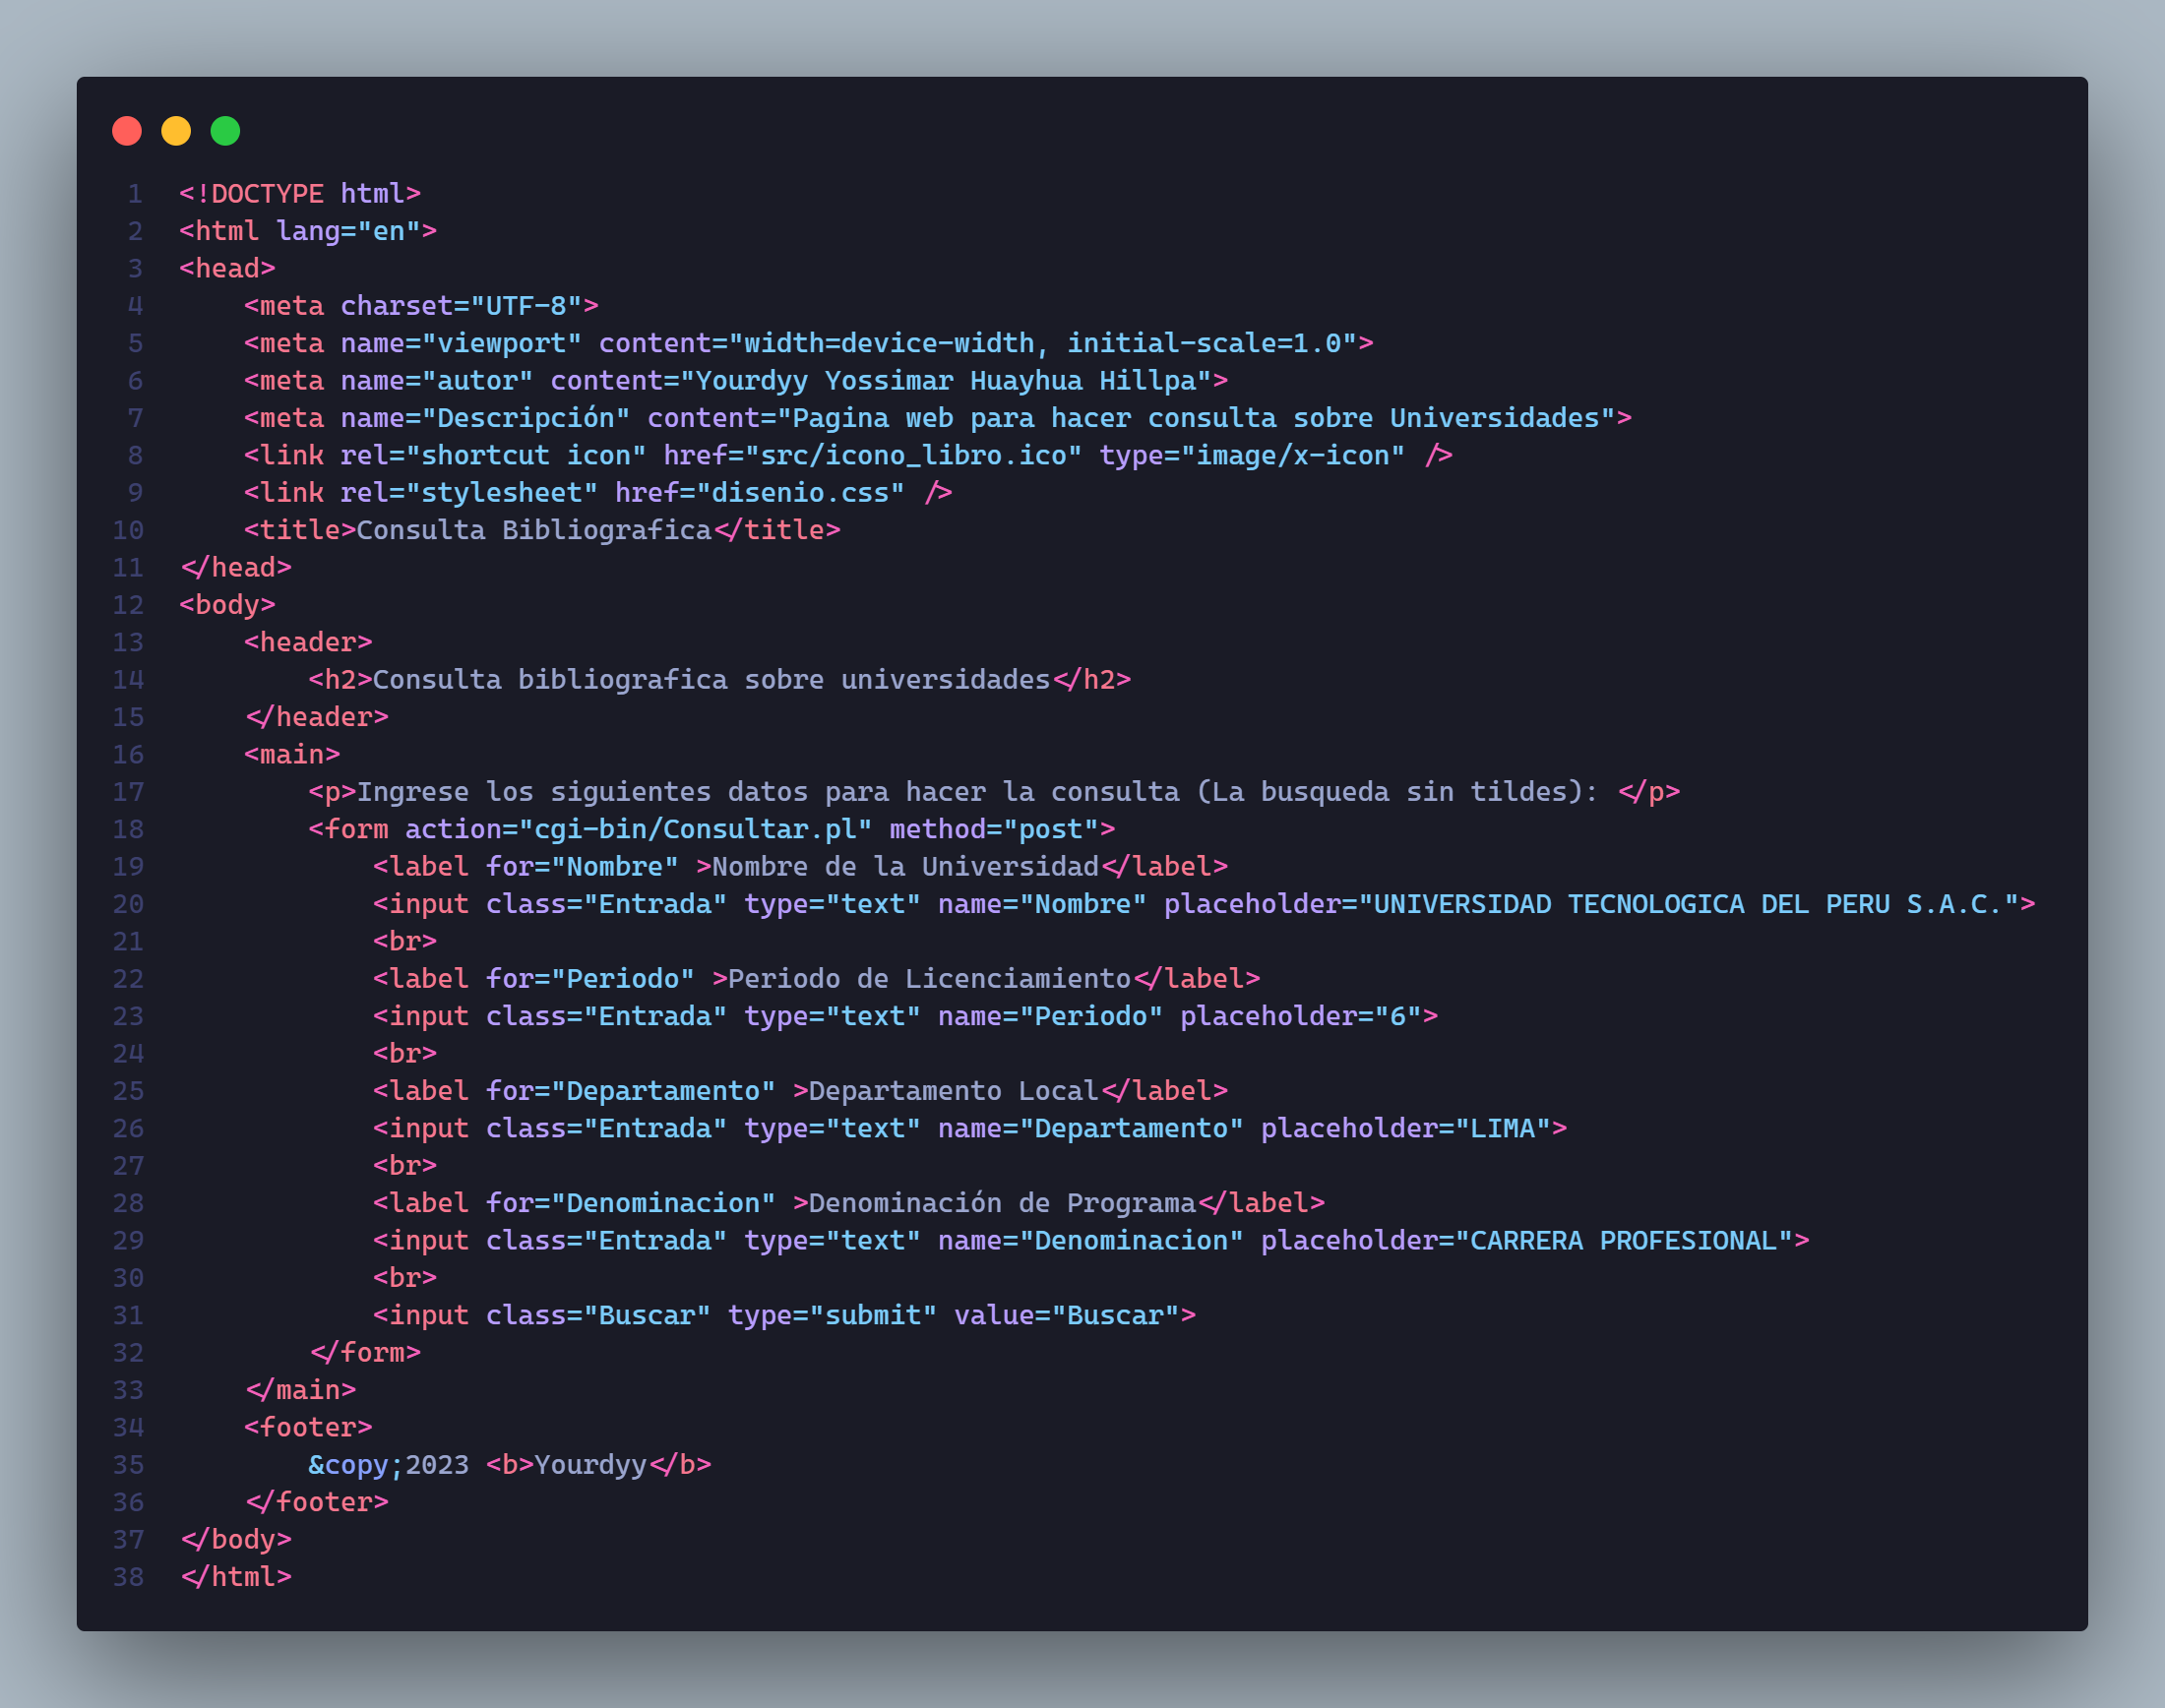
\includegraphics[width=1.0\textwidth,keepaspectratio]{img/Consulta_html.png}
    %\includesvg{img/automata.svg}
    %\label{img:mot2}
    %\caption{Product backlog.}
\end{figure}\\

\subsection{Codigo Fuente : disenio.css}
%\lipsum[5]
Ahora el codigo del diseño de las paginas web: 
\begin{figure}[h!]
    \centering
    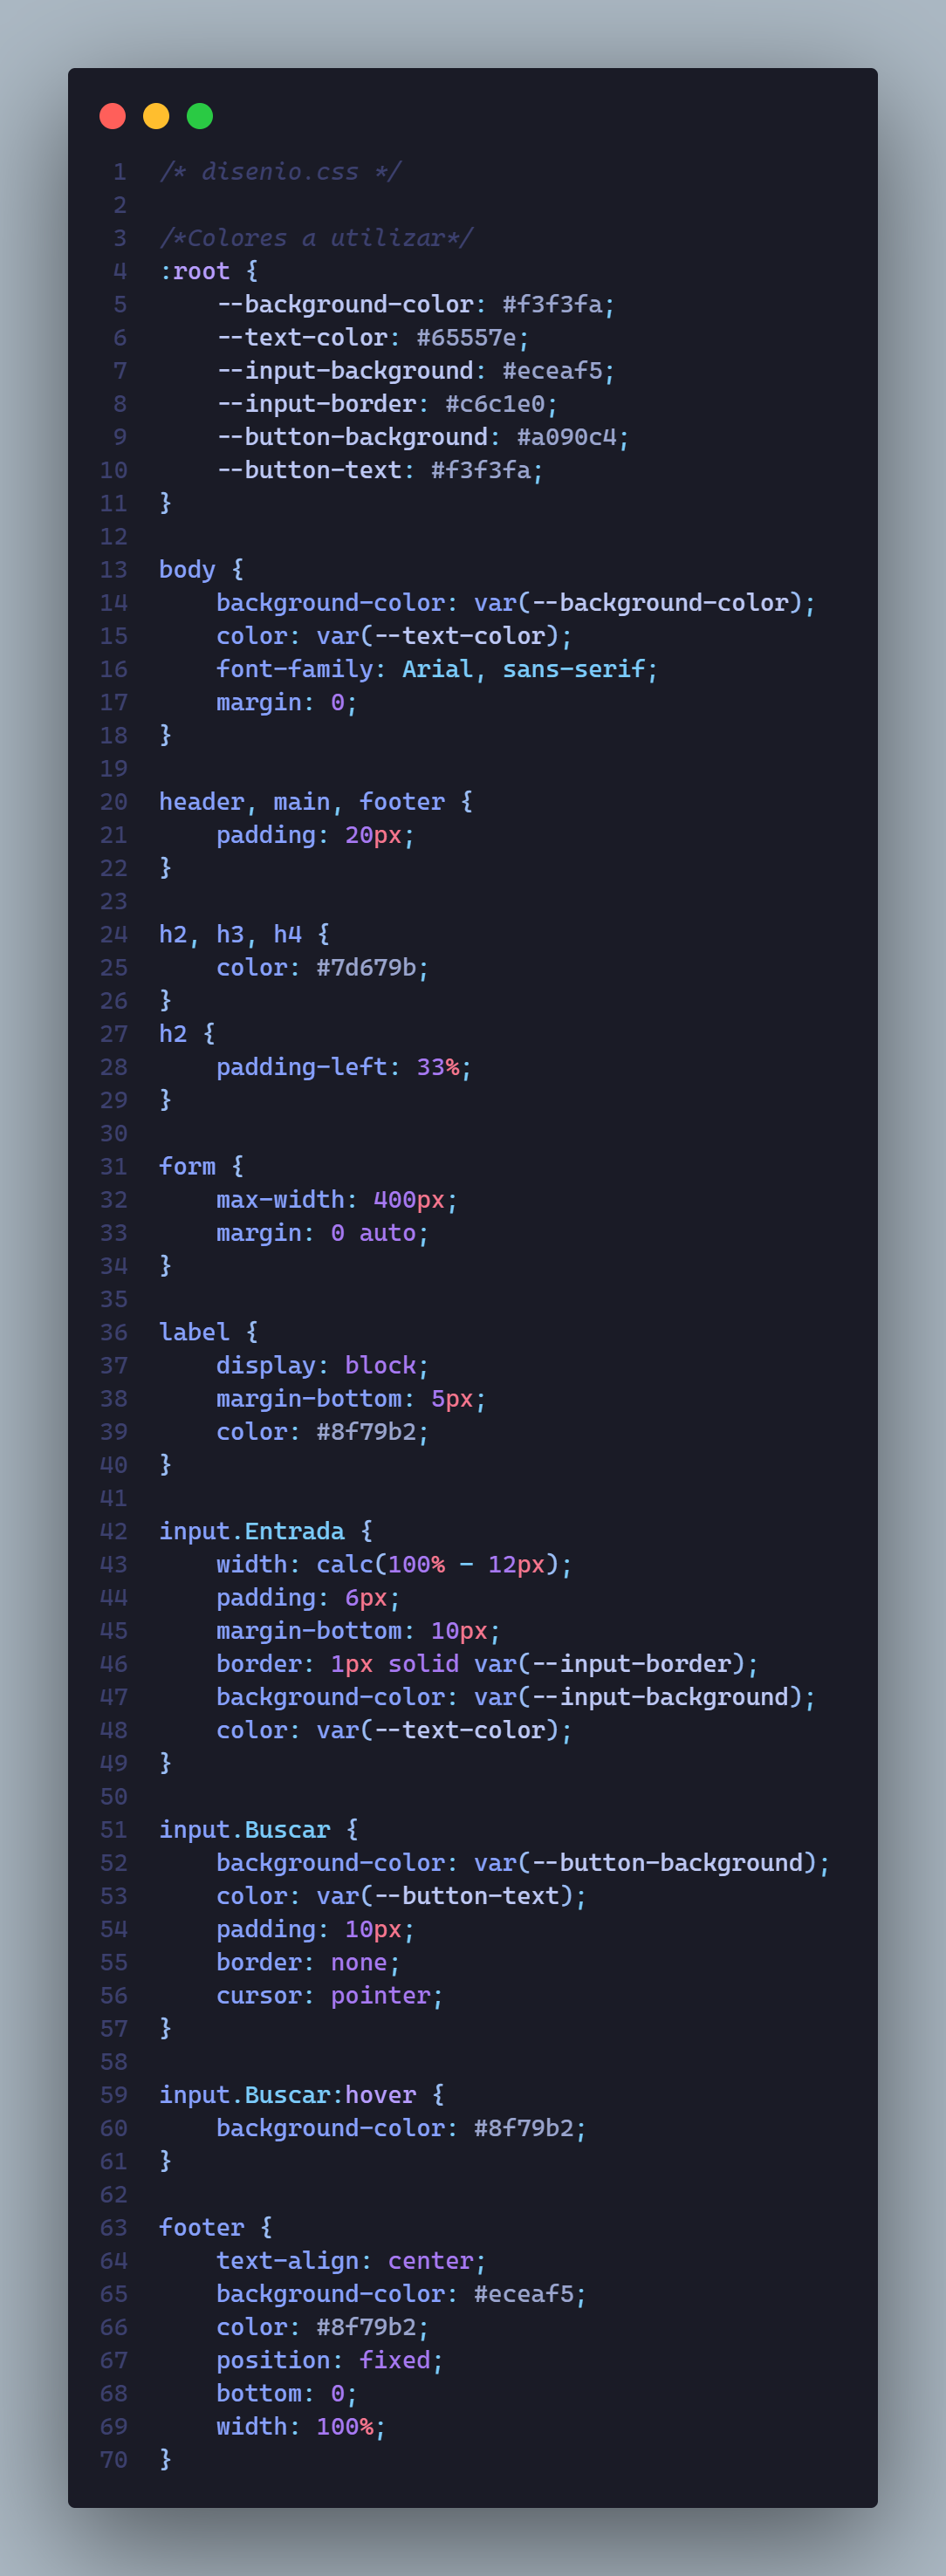
\includegraphics[width=0.5\textwidth,keepaspectratio]{img/disenio_css.png}
    %\includesvg{img/automata.svg}
    %\label{img:mot2}
    %\caption{Product backlog.}
\end{figure}
\clearpage

\subsection{Codigo Fuente : Consultar.pl}

Por ultimo el codigo del programa que maneja el archivo .csv:
\begin{figure}[h!]
    \centering
    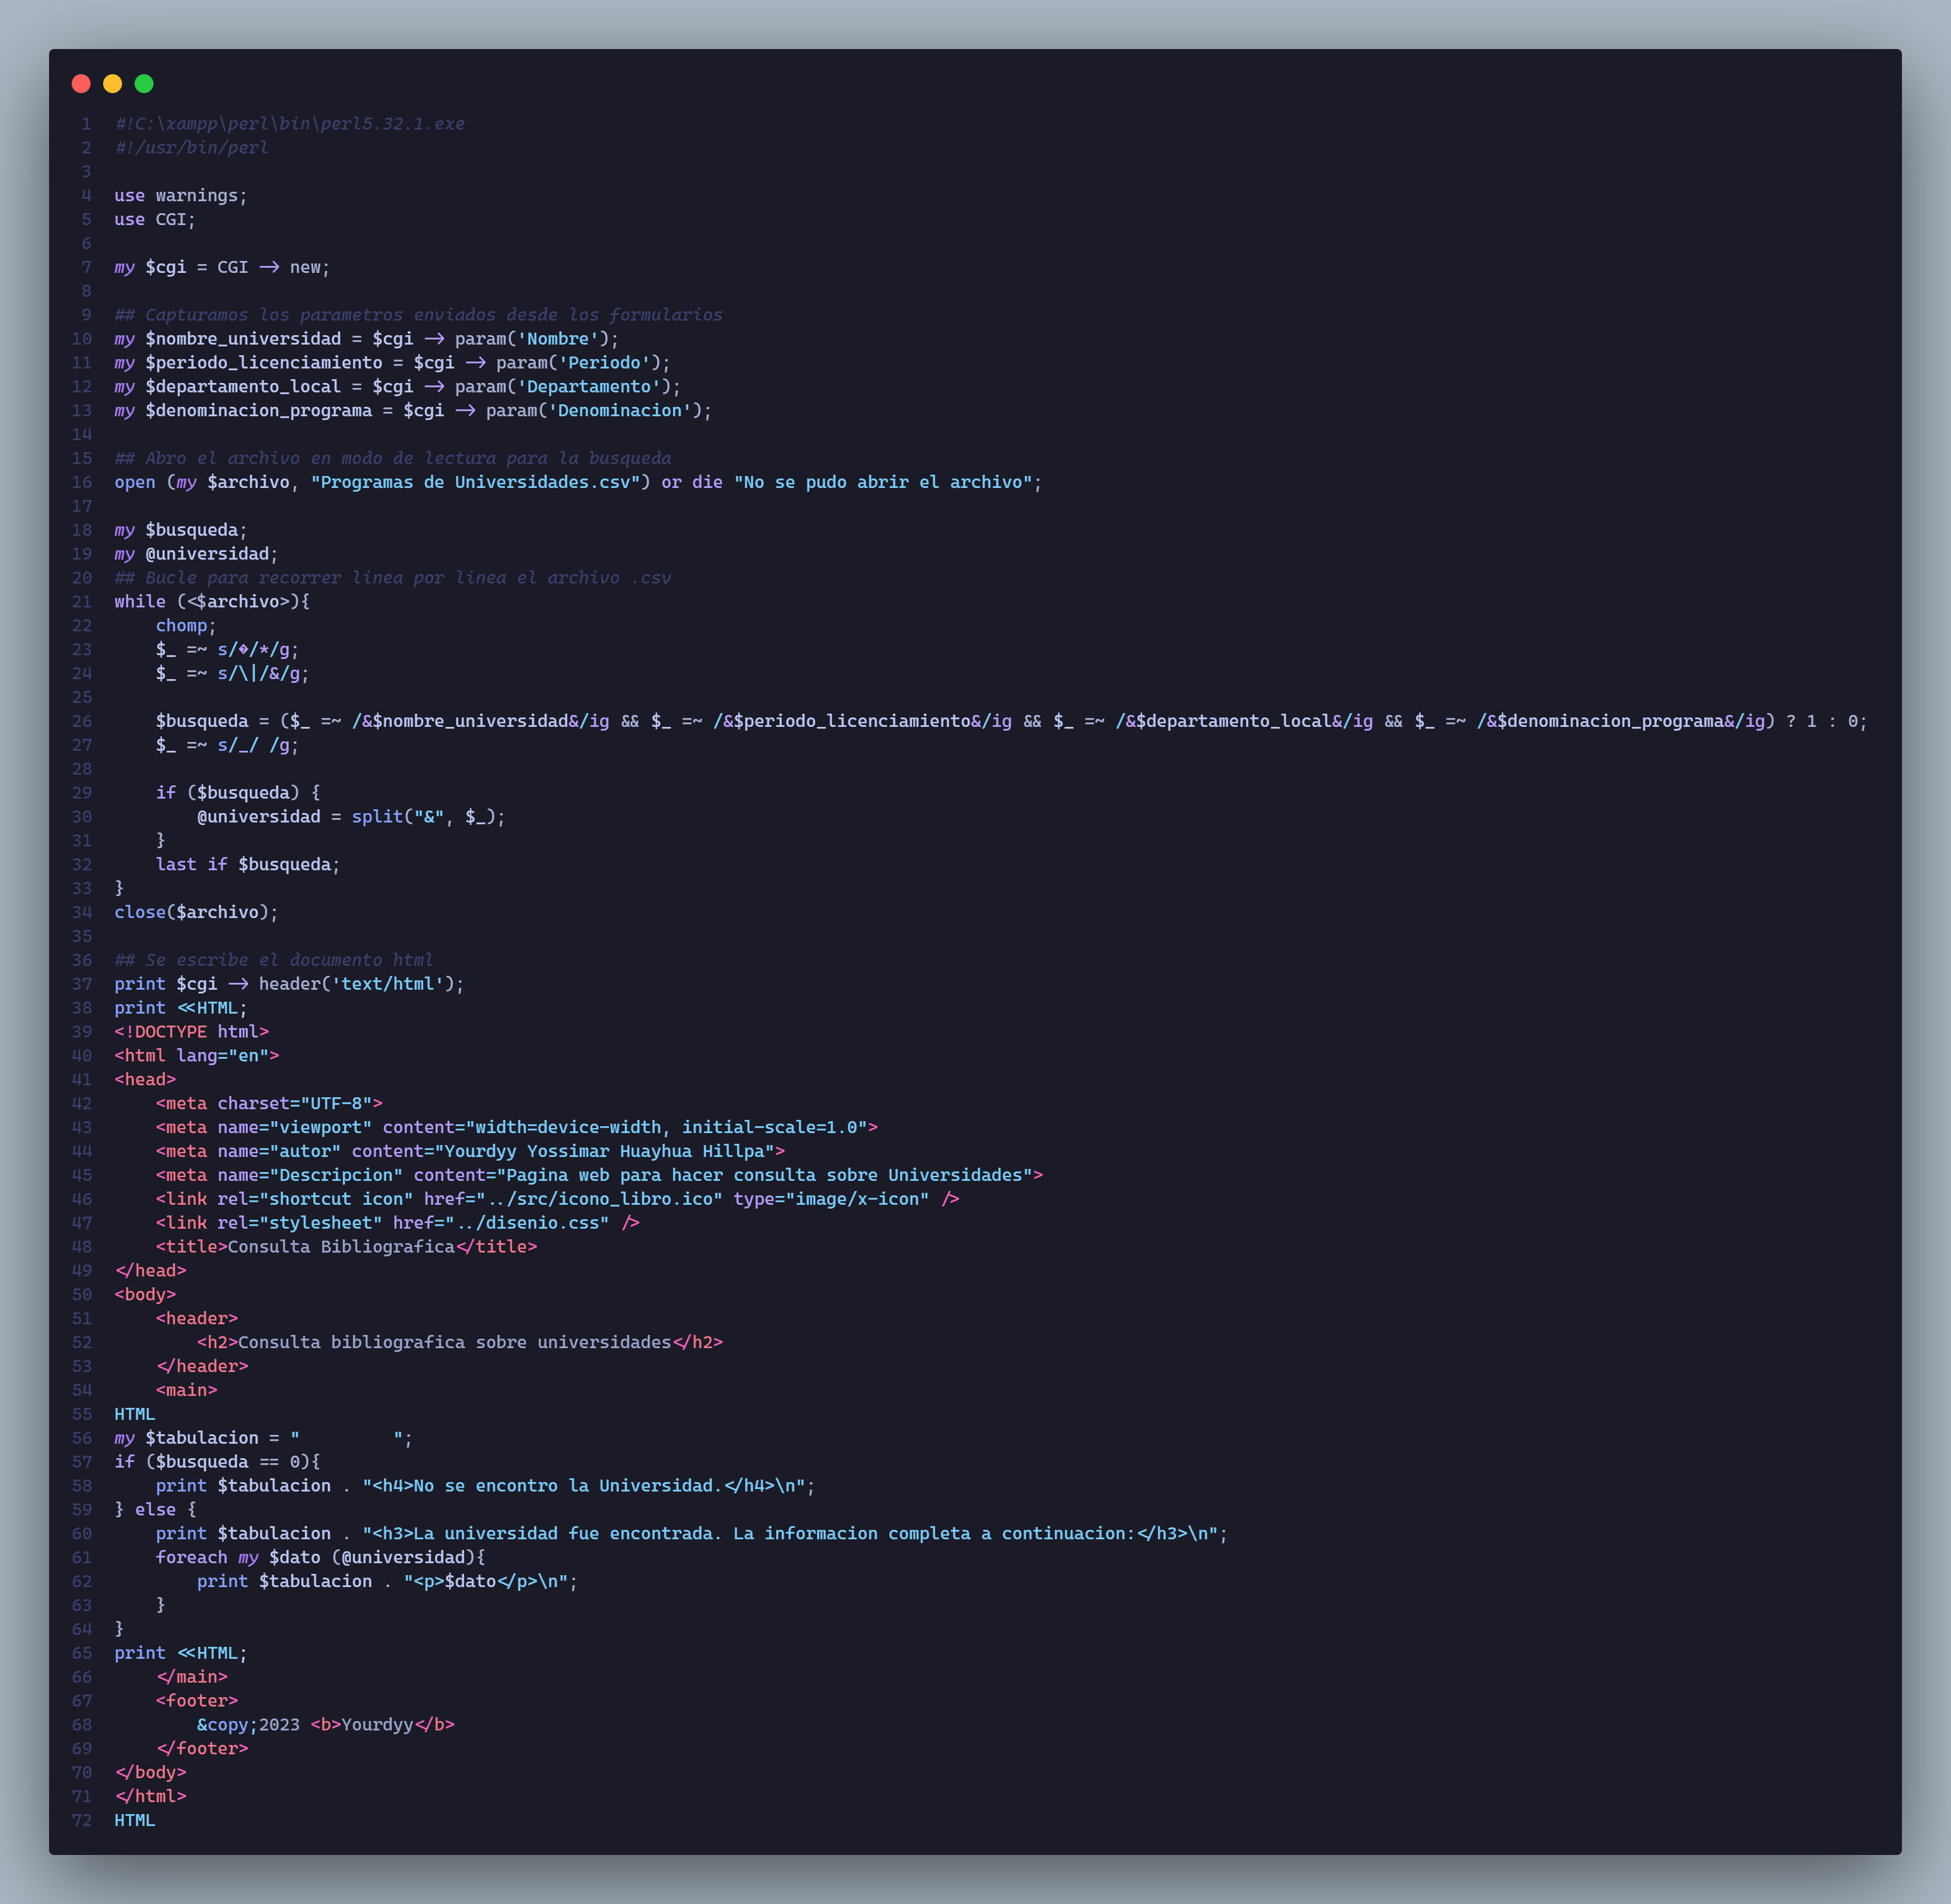
\includegraphics[width=1.2\textwidth,keepaspectratio]{img/Consultar_pl.png}
    %\includesvg{img/automata.svg}
    %\label{img:mot2}
    %\caption{Product backlog.}
\end{figure}
\clearpage

\subsection{Estructura del Laboratorio y Repositorio:}

La estructura del laboratorio es de la siguiente manera:
\begin{figure}[h!]
    \centering
    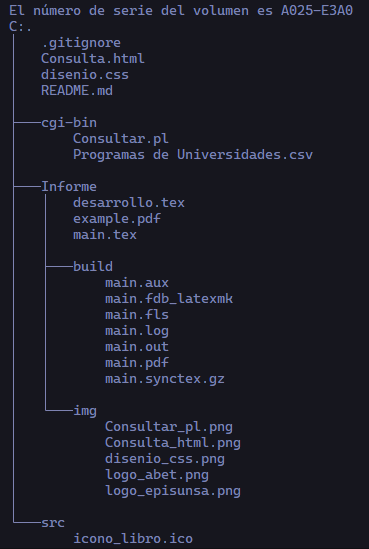
\includegraphics[width=0.6\textwidth,keepaspectratio]{img/Estructura.png}
    %\includesvg{img/automata.svg}
    %\label{img:mot2}
    %\caption{Product backlog.}
\end{figure}
\\
Repositorio GitHub:
\url{https://github.com/yhuayhuahi/Lab_09.git}

\subsection{Prueba del programa}
Capturas de pantalla, de como se muestra en el navegador:
\begin{figure}[h!]
    \centering
    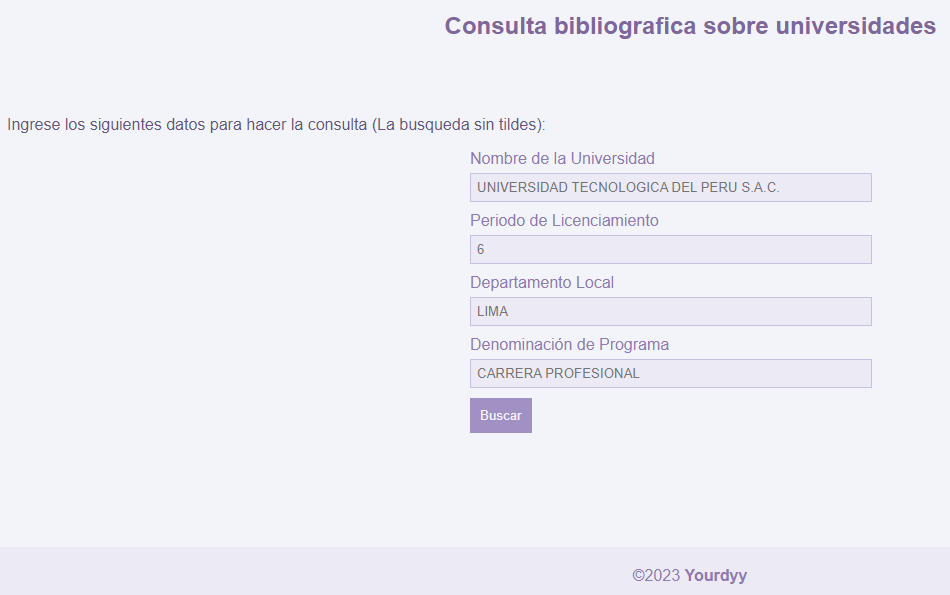
\includegraphics[width=0.8\textwidth,keepaspectratio]{img/Prueba1.png}
    %\includesvg{img/automata.svg}
    %\label{img:mot2}
    %\caption{Product backlog.}
\end{figure}
\begin{figure}[h!]
    \centering
    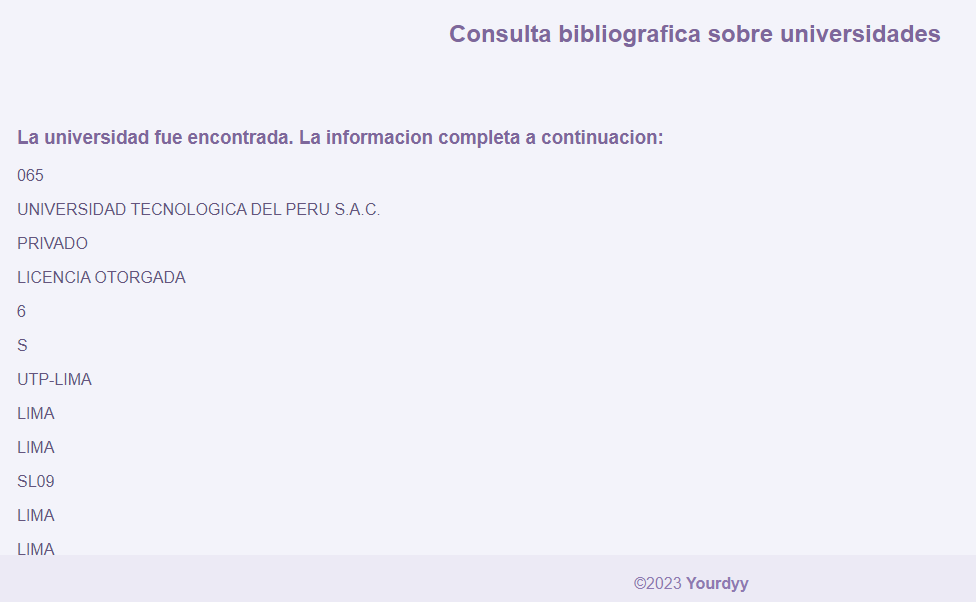
\includegraphics[width=0.8\textwidth,keepaspectratio]{img/Prueba2.png}
    %\includesvg{img/automata.svg}
    %\label{img:mot2}
    %\caption{Product backlog.}
\end{figure}
\begin{figure}[h!]
    \centering
    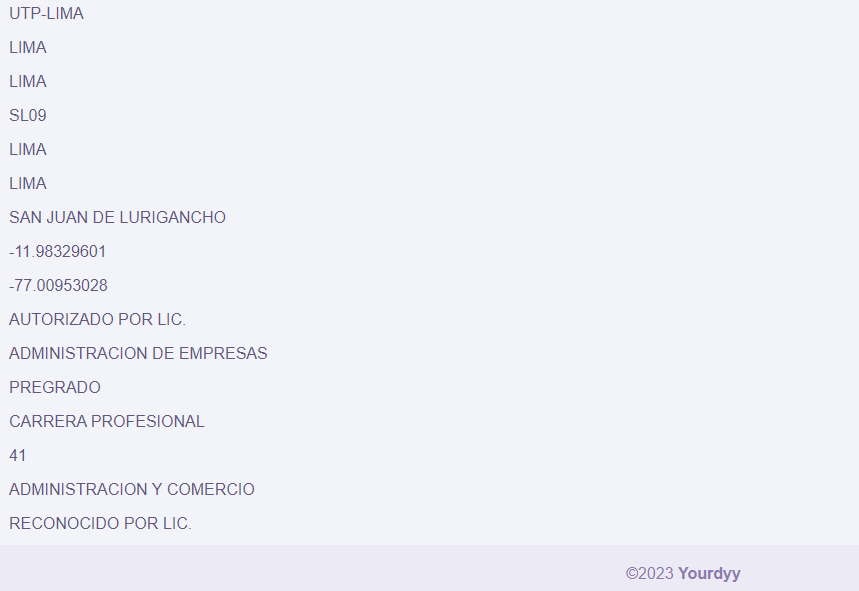
\includegraphics[width=0.8\textwidth,keepaspectratio]{img/Prueba3.png}
    %\includesvg{img/automata.svg}
    %\label{img:mot2}
    %\caption{Product backlog.}
\end{figure}

%\section*{REFERENCIAS}
%\begin{itemize}
%    \item https://www.w3schools.com/c/index.php
%    \item https://www.w3schools.com/cpp/default.asp
%\end{itemize}

 % Desarrolla tu contenido dentro de desarrollo
    %\input{conclusiones} % agregar las partes necesarias
    
\end{document}